\documentclass[11pt]{beamer}
\usetheme{CambridgeUS}
\usepackage[utf8]{inputenc}
\usepackage{amsmath}
\usepackage{amsfonts}
\usepackage{amssymb}
\usepackage[capposition=top]{floatrow}
\usepackage{float}
\usepackage{caption}
\usepackage{pgfpages}
\usepackage{graphicx}
\usepackage{subfig}
\usepackage{listings}
\usepackage{multicol}

\newcommand*{\itemimg}[1]{%
  \raisebox{-.3\baselineskip}{%
    \includegraphics[
      height=\baselineskip,
      width=\baselineskip,
      keepaspectratio,
    ]{#1}%
  }%
}

\pgfpagesuselayout{resize to}[a4paper,landscape,border shrink=5mm]

\author{Giovanni Della Lunga}
\title{Introduction to Monte Carlo in Finance}
%\setbeamercovered{transparent} 
%\setbeamertemplate{navigation symbols}{} 
%\logo{} 
%\institute{Università degli Studi di Bologna}
%\institute{Scuola di Economia, Management e Statistica} 
\institute{WORKSHOP IN QUANTITATIVE FINANCE} 
\date{Bologna - May 3-4, 2018} 
\begin{document}

\begin{frame}
\titlepage
\end{frame}

\AtBeginSection[]
{
\begin{frame}<beamer>
  %\footnotesize	
  \frametitle{Outline}
  %\begin{multicols}{2}
  \tableofcontents[currentsection]
  %\end{multicols}	  
  %\normalsize
\end{frame}
}

%===================================================================================================
\section{Valuation of American Option}
%...................................................................................................
\begin{frame}{Valuation of American Option by Simulation}
\begin{itemize}
\item As we have seen Monte Carlo simulation is a flexible and powerful numerical method to value financial derivatives of any kind. 
\item However being a forward evolving technique, it is per se not suited to address the valuation of American or Bermudan options which are valued in general by backwards induction. 
\item Longstaff and Schwartz provide a numerically efficient method to resolve this problem by what they call Least-Squares Monte Carlo. 
\item  The problem with Monte Carlo is that the decision to exercise an American option or not is dependent on the continuation value. 
\end{itemize}
\end{frame}
%...................................................................................................
\begin{frame}{Valuation of American Option by Simulation}
\begin{itemize}
\item  Consider a simulation with $M + 1$ points in time and $I$ paths. 
\item Given a simulated index level $S_{t,i} , t\in \{0, ..., T \}, i \in \{1, ..., I \}$, what is the continuation value $C_{t,i}(S_{t,i})$, i.e. the expected payoff of not exercising the option? 
\item The approach of Longstaff-Schwartz approximates continuation values for American options in the backwards steps by an ordinary least-squares regression.
\item Equipped with such approximations, the option is exercised if the approximate continuation value is lower than the value of immediate exercise. Otherwise it is not exercised.
\end{itemize}
\end{frame}
%...................................................................................................
\begin{frame}{Valuation of American Option by Simulation}
\begin{itemize}
\item In order to explain the metodology, let's start from a simpler problem. 
\item Consider a bermudan option which is similar to an american option, except that it can be early exercised once only on a specific set of dates. 
\item In the next figure, we can represent the schedule of a put bermudan option with strike $K$ and maturity in $6$ years. Each year you can choose whether to exercise or not ...
\end{itemize}
\end{frame}
%...................................................................................................
\begin{frame}{Valuation of American Option by Simulation}
\begin{center}
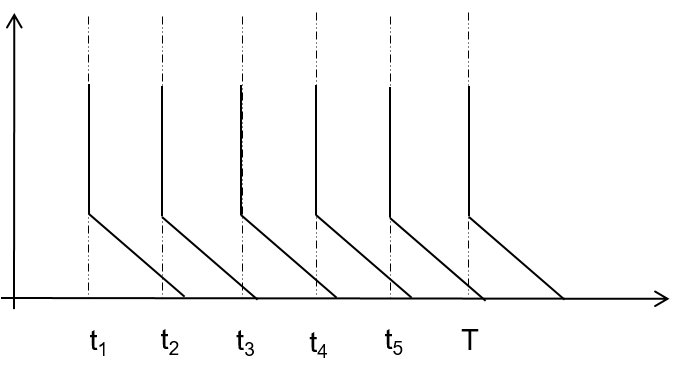
\includegraphics[scale=1]{img/bermudan_exercise_1.png} 
\end{center}
\end{frame}
%...................................................................................................
\begin{frame}{Valuation of American Option by Simulation}
\begin{itemize}
\item Let's consider a simpler example: a put option which can be exercised early only once ... 
\end{itemize}
\end{frame}
%...................................................................................................
\begin{frame}{Valuation of American Option by Simulation}
\begin{center}
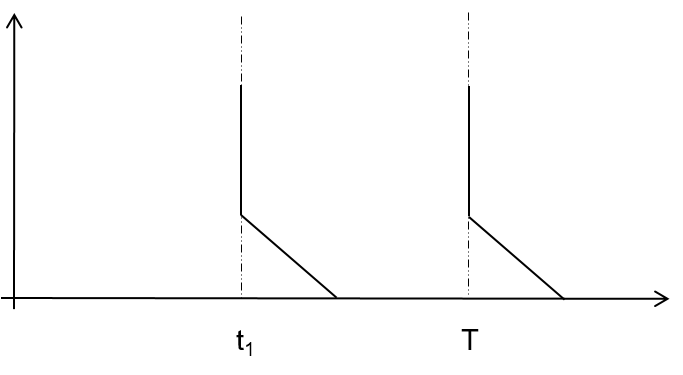
\includegraphics[scale=1]{img/bermudan_exercise_2.png} 
\end{center}
\end{frame}
%...................................................................................................
\begin{frame}{Valuation of American Option by Simulation}
\begin{itemize}
\item Can we price this product by means of a Monte Carlo? Yes we can! Let's see how.

\item Let's implement a MC which actually simulates, besides the evolution of the market, what an investor holding this option would do (clearly an investor who lives in the risk neutral world). In the following example we will assume the following data, $S(T)=$, $K=$, $r=$, $\sigma=$, $t_1=1y$, $T=2y$.

\item We simulate that 1y has passed, computing the new value of the asset and the new value of the money market account

$$S(t_1 = 1y) = S(t_0)e^{(r-\frac{1}{2}\sigma^2 )(t_1-t_0) + \sigma \sqrt{t_1-t_0}N(0,1)}$$

$$B(t_1 = 1y) = B(t_0) e^{r(t_1-t_0)}$$

\end{itemize}
\end{frame}
%...................................................................................................
\begin{frame}{Valuation of American Option by Simulation}
\begin{itemize}
\item At this point the investor could exercise. How does he know if it is convenient? 
\item In case of exercise he knows exactly the payoff he's getting. 
\item In case he continues, he knows that it is the same of having a European Put Option.

\item So, in mathematical terms we have the following payoff in $t_1$

$$\max \left[
K-S(t_1), P(t_1,T;S(t_1),K)
\right] $$

where $P(t_1,T;S(t_1),K)$ is the price of a Put which we compute analytically! 
\item In the jargon of american products, $P$ is called the continuation value, i.e. the value of holding the option instead of early exercising it.

\end{itemize}
\end{frame}
%...................................................................................................
\begin{frame}{Valuation of American Option by Simulation}
\begin{itemize}
\item So the premium of the option is the average of this discounted payoff calculated in each iteration of the Monte Carlo procedure.

$$
\frac{1}{N} \sum\limits_i
\max \left[
K-S_i(t_1), P(t_1,T;S_i(t_1),K)
\right] $$

\item Some considerations are in order. 
\item We could have priced this product because we have an analytical pricing formula for the put. What if we didn't have it? 

\end{itemize}
\end{frame}
%...................................................................................................
\begin{frame}{Valuation of American Option by Simulation}
\begin{itemize}
\item Brute force solution: for each realization of $S(t_1)$ we run another Monte Carlo to price the put. 
\item This method (called Nested Monte Carlo) is very time consuming. For this very simple case it's time of execution grows as $N^2$, which becomes prohibitive when you deal with more than one exercise date!

\item Let's search for a finer solution analyzing the relationship between the continuation value (in this very simple example) and the simulated realization of $S$ at step $t_1$. 
\item let's plot the discounted payoff at maturity, $P_i$, versus $S_i(t_1)$ ... 
\end{itemize}
\end{frame}
%...................................................................................................
\begin{frame}{Valuation of American Option by Simulation}
\begin{center}
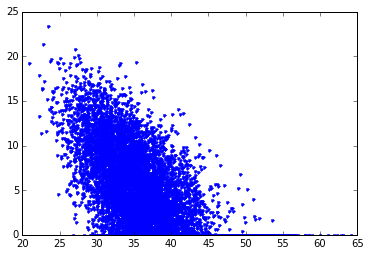
\includegraphics[scale=.8]{img/lsm_1.png} 
\end{center}
\end{frame}
%...................................................................................................
\begin{frame}{Valuation of American Option by Simulation}
\begin{center}
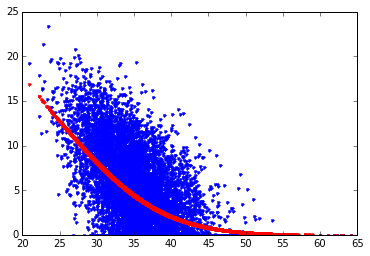
\includegraphics[scale=.8]{img/lsm_2.png} 
\end{center}
\end{frame}
%...................................................................................................
\begin{frame}
\begin{itemize}
\item As you can see, the analytical price of the put is a curve which kinds of interpolate the cloud of Monte Carlo points. \item This suggest us that
the price at time $t_1$ can be computed by means of an average on all discounted payoff (i.e. the barycentre of the cloud made of discounted payoff)
\item So maybe...
the future value of an option can be seen as the problem of finding the curve that best fits the cloud of discounted payoff (up to date of interest)!!!
\item In the next slide, for example, there is a curve found by means of a linear regression on a polynomial of 5th order...
\end{itemize}
\end{frame}
%...................................................................................................
\begin{frame}{Valuation of American Option by Simulation}
\begin{center}
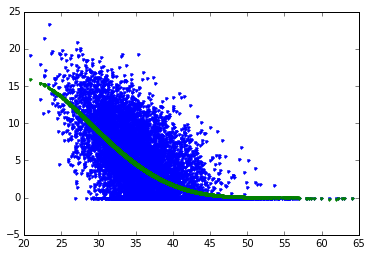
\includegraphics[scale=.8]{img/lsm_3.png} 
\end{center}
\end{frame}
%...................................................................................................
\begin{frame}{Valuation of American Option by Simulation}
\begin{center}
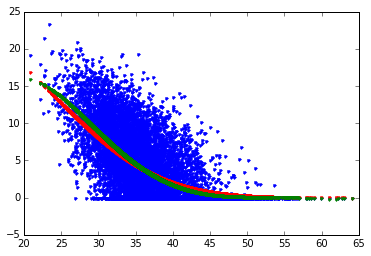
\includegraphics[scale=.8]{img/lsm_4.png} 
\end{center}
\end{frame}
%...................................................................................................
\begin{frame}{Valuation of American Option by Simulation}
\begin{itemize}
\item We now have an empirical pricing formula for the put to be used in my MCS
\footnotesize
$$P(t_1, T, S(t_1), K) = c_0 + c_1S(t_1) + c_2S(t_1)^2 + c_3S(t_1)^3 + c_4S(t_1)^4 + c_5S(t_1)^5$$
\normalsize
\item The formula is obviously fast, the cost of the algorithm being the best fit. 
\item Please note that we could have used any form for the curve (not only a polynomial). 
\item This method has the advantage that it can be solved as a linear regression, which is fast.
\end{itemize}
\end{frame}
%...................................................................................................
\begin{frame}{The Longstaff-Schwartz Algorithm}
\begin{itemize}
\item The major insight of Longstaff-Schwartz is to estimate the continuation value $C_{t,i}$ by ordinary least-squares regression, therefore the name "Least Square Monte Carlo" for their algorithm;
\item They propose to regress the $I$ continuation values $Y_{t,i}$ against the $I$ simulated index levels $S_{t,i}$. \item Given $D$  basis functions $b$ with $b_1, \dots, b_D : \mathbb{R}^D \rightarrow \mathbb{R}$ for the regression, the continuation value $C_{t,i}$ is according to their approach approximated by: 
\end{itemize}
\end{frame}
%...................................................................................................
\begin{frame}{The Longstaff-Schwartz Algorithm}
\begin{itemize}
\item Given $D$  basis functions $b$ with $b_1, \dots, b_D : \mathbb{R}^D \rightarrow \mathbb{R}$ for the regression, the continuation value $C_{t,i}$ is according to their approach approximated by: 
$$
\hat C_{t,i} = \sum\limits_{d=1}^D \alpha^\star_{d,t} b_d(S_{t,i})  \quad (1)
$$
\item The optimal regression parameters $\alpha^\star_{d,t}$ are the result of the minimization 

$$
\min\limits_{\alpha_{1,t}, \dots, \alpha_{D,t}}   \frac{1}{I} \sum\limits_{i=1}^I 
\left( Y_{t,i} - \sum\limits_{d=1}^D \alpha_{d,t} b_d(S_{t,i}) \right)^2
$$

\end{itemize}
\end{frame}
%...................................................................................................
\begin{frame}{The Longstaff-Schwartz Algorithm}
\begin{itemize}
\item Simulate $I$ index level paths with $M + 1$ points in time leading to index level values 
$S_{t,i} , t\in \{0, ..., T \}, i \in \{1, ..., I \}$;
\item  For $t=T$ the option value is $V_{T,i} = h_T(S_{T,i})$ by arbitrage
\item  Start iterating backwards $t = T - \Delta t , \dots, \Delta t$:
\begin{itemize}
    \item regress the $T_{t,i}$ against the $S_{t,i}, i \in \{1, \dots, I\}$, given $D$ basis function $b$
    \item approximate $C_{t,i}$ by $\hat C_{t,i}$ according to (1) given the optimal parameters $\alpha^\star_{d,t}$ from       (2)
    \item set 
    $$V_{t,i}= 
    \begin{cases}
      h_t(S_{t,i})       & \quad \text{if } h_t(S_{t,i}) >   \hat C_{t,i} \quad \text{exercise takes place}\\
      Y_{t,i}            & \quad \text{if } h_t(S_{t,i}) \le \hat C_{t,i} \quad \text{no exercise takes place}\\
    \end{cases}
    $$
\end{itemize}    
  repeat iteration steps until $t=\Delta t$;
\item for $t=0$ calculate the LSM estimator
$$
\hat V_0^{LSM} = e^{-r \Delta t} \frac{1}{I}  \sum\limits_{i=1}^I V_{\Delta t,i} 
$$
\end{itemize}
\end{frame}
%...................................................................................................
\begin{frame}{Notebook}
\noindent\begin{minipage}{0.5\textwidth}% adapt widths of minipages to your needs

\includegraphics[width=\linewidth]{img/exercise.jpg}
\end{minipage}%
\hfill%
\begin{minipage}{0.5\textwidth}
\begin{itemize}
\item {\bf GitHub        : }    polyhedron-gdl;
\item {\bf Notebook   : }    mcs\_american;
\end{itemize}
\end{minipage}
\end{frame}
%===================================================================================================
\section{The Hull and White Model}
%...................................................................................................
\begin{frame}{Hull-White Model}
\begin{itemize}
\item Described by the SDE for the short rate
\begin{equation}\label{HW SDE}
dr = (\theta(t) - ar)dt + \sigma dw
\end{equation}
\item See Brigo-Mercurio ...
\item Our version simplified: $a$ and $\sigma$ constant;
\item AKA Extended Vasicek (Note: $r(t)$ is Gaussian);
\item $\theta$ determined uniquely by term structure;
\end{itemize}
\end{frame}
%...................................................................................................
\begin{frame}{Hull-White Model: Solving for r(t)}
$$
d(e^{at} r) = e^{at} dr + ae^{at}rdt = \theta(t) e^{at} + e^{at} \sigma dw
$$
integrating both sides we obtain
$$
e^{at} r(t) = r(0) + \int\limits_{0}^t \theta(s) e^{as} ds + \sigma \int\limits_0^t e^{as} dw(s)
$$
simplify
$$
 r(t) = r(0)e^{-at} + \int\limits_{0}^t \theta(s) e^{-a(t-s)} ds + \sigma \int\limits_0^t e^{-a(t-s)} dw(s)
$$
\end{frame}
%...................................................................................................
\begin{frame}{Hull-White Model: Solving for P(t,T)}
\begin{itemize}
\item $P(t,T) = V(t, r(t))$ where $V$ solves the PDE
$$
V_t + (\theta(t) - ar) V_r + \frac{1}{2} \sigma^2 V_{rr} - rV = 0
$$
\item Final-time condition $V(T,r) = 1$ for all $r$ at $t=T$;
\item Ansatz: 
$$
V=A(t,T) e^{-B(t,T)r(t)}
$$
\item $A$ and $B$ must satisfy:
$$
A_t - \theta(t) AB + \frac{1}{2} \sigma^2 (AB)^2 = 0, \quad and \quad B_t -aB +1 = 0
$$
\item Final-time conditions
$$A(T,T) =1 \quad and \quad B(T,T)=0$$
\end{itemize}
\end{frame}
%...................................................................................................
\begin{frame}{Hull-White Model: Solving for P(t,T)}
\begin{itemize}
\item $B$ independent of $\theta$ so
\begin{equation}
B(t,T) = \frac{1}{a} \left( 1 - e^{-a(T-t)} \right)
\end{equation}
\item Solving for $A$ requires integration of $\theta$
\footnotesize
$$
A(t,T) = exp \left[  -\int\limits_t^T \theta(s) B(s,T) ds - 
\frac{\sigma^2}{2a^2} \left( B(t,T) - T + t \right)  -
\frac{\sigma^2}{4a} B(t,T)^2 \right]
$$
\normalsize
\end{itemize}
\end{frame}
%...................................................................................................
\begin{frame}{Hull-White Model: Determining $\theta$} 
\begin{itemize}
\item Determining $\theta$ from the term structure at time $0$;
\item Goal: demonstrate the relation
\begin{equation}
\theta(t) = \frac{\partial f}{f\partial T}(0,t) +a f(0,t) + \frac{\sigma^2}{2a}(1-e^{-2at})
\end{equation}
\item Recall
$$
f(t,T) = -\partial \log P(t,T) / \partial T
$$
\end{itemize}
\end{frame}
%...................................................................................................
\begin{frame}{Hull-White Model: Determining $\theta$}
\begin{itemize}
\item We have
\footnotesize
$$
-\log P(0,T) = \int\limits_0^T \theta(s) B(s,T) ds  + \frac{\sigma^2}{2a^2}   [B(0,T) - T] + \frac{\sigma^2}{4a} B(0,T)^2 + B(0,T) r_0
$$
\normalsize
\item Differentiating and using that $B(T,T)=1$ and $\partial_T B - 1 = -aB$ we get
\footnotesize
$$
f(0,T) = \int\limits_0^T \theta(s) \partial_T B(s,T) ds - \frac{\sigma^2}{2a^2}   B(0,T) + \frac{\sigma^2}{2a^2}   B(0,T) \partial_T B(0,T) + \partial_T B(0,T) r_0
$$
\normalsize
\end{itemize}
\end{frame}
%...................................................................................................
\begin{frame}{Hull-White Model: Determining $\theta$}
\begin{itemize}
\item Differentiating again, get:
\begin{equation}
\begin{split}
\partial_T f(0,T) &= \theta(T) + \int\limits_0^T \theta(s) \partial_{TT} B(s,T) ds  \\
&- \frac{\sigma^2}{2a^2} \partial_T B(0,T) \\ 
&+ \frac{\sigma^2}{2a^2} [(\partial_T B(0,T))^2 + B(0,T) \partial_{TT} B(0,T)] \\
&+ \partial_{TT} B(0,T) r_0 
\end{split}
\end{equation}
\end{itemize}
\end{frame}
%...................................................................................................
\begin{frame}{Hull-White Model: Determining $\theta$}
\begin{itemize}
\item Combine these equations, and use $a \partial_T B + \partial_{TT} B = 0$;
\item Get:
\footnotesize
$$
af(0,T) + \partial_T f(0,T) = \theta(T) - \frac{\sigma^2}{2a} (aB + \partial_T B) +
\frac{\sigma^2}{2a} [aB \partial_T B + (\partial_T B)^2 + B \partial_{TT}B] 
$$
\normalsize
\item Substitute formula for $B$ and simplify to get
$$
af(0,T) + \partial_T f(0,T) = \theta(T) - \frac{\sigma^2}{2a} (1 - e^{-2aT})
$$
QED
\end{itemize}
\end{frame}
%...................................................................................................
\begin{frame}{Additive Factor Gaussian Model}
\begin{itemize}
\item The model is given by dynamics (Brigo-Mercurio p. 143):
$$r(t) = x(t) + \phi(t)$$
where
$$dx(t) = - a x(t)dt+\sigma dW_t \quad x(0)=0$$
and $\phi$ is a deterministic shift which is added in order to fit exactly the initial zero coupon curve
\end{itemize}
\end{frame}
%...................................................................................................
\begin{frame}{Additive Factor Gaussian Model}
\begin{itemize}
\item So the short rate $r(t)$ is distributed normally with mean and variance given by (Brigo-Mercurio p.144 equations 4.6 with $\eta = 0$)

$$
E(r_t \vert r_s)= x(s) e^{-a(t-s)} + \phi(t)
$$

$$
Var(r_t \vert r_s) = \frac{\sigma^2}{2a} \left( 1-e^{-2a(t-s)} \right)
$$

where $\phi(T) = f^M(0,T) + \frac{\sigma^2}{2a} \left( 1-e^{-aT} \right)^2$ and $f^M(0,T)$ is the market instantaneous forward rate at time $t$ as seen at time $0$.
\end{itemize}
\end{frame}
%...................................................................................................
\begin{frame}{Additive Factor Gaussian Model}
\begin{itemize}
\item Model discount factors are calculated as in Brigo-Mercurio (section 4.2): 

$$P(t,T)=\frac{P^M(0,T)}{P^M(0,t)}\exp\left( \mathcal{A}(t,T) \right) $$ 
$$\mathcal{A}(t,T) = \frac{1}{2} \left[ V(t,T) - V(0,T) + V(0,t) \right] - \frac{1-e^{-a(T-t)}}{a}x(t)
$$ 

where

$$V(t,T) = \frac{\sigma^2}{a^2} \left[
T-t+\frac{2}{a}e^{-a(T-t)}-\frac{1}{2a} e^{-2a(T-t)} - \frac{3}{2a}
\right]
$$
\end{itemize}
\end{frame}
%===================================================================================================
\section{MCS for CVA Estimation}
%...................................................................................................
%...................................................................................................
\subsection{Definitions}
%...................................................................................................
%...................................................................................................
%...................................................................................................
\begin{frame}{Counterparty Risk}
\begin{itemize}
\item In general a given company, say a financial institution A, will have portfolios
with many other counterparties, varying among sovereign entities, corporates, hedge
funds, insurance companies;
\item Counterparty credit exposure is the amount a company, say A, could potentially
lose in the event of one of its counterparties defaulting. 
\item As we'll see in more details, it can be computed by simulating
in different scenarios and at different times in the future, the price of the transactions with the given counterparty, and then by using some chosen statistic to
characterise the price distributions that have been generated.
\end{itemize}
\end{frame}
%...................................................................................................
\begin{frame}{CVA Context}
\begin{itemize}
\item Counterparty risk can be considered broadly from two different points of view;
\item The first point of view is risk management, leading to capital requirements revision, trading limits discussions and so on;
\item The second point of view is valuation or pricing, leading to amounts called Credit Valuation Adjustment (CVA) and extensions thereof, including netting, collateral, re-hypothecation, close-out specification, wrong way risk and funding cost;
\end{itemize}
\end{frame}
%...................................................................................................
\begin{frame}{Example: CVA of plain vanilla Interest-Rate Swap}
\begin{itemize}
\item Consider counterparties A and B who enter into an interest-rate swap where A receives
every six months the 6-month Libor rate on a notional of $100$ million euro, while
paying to B a fixed amount equal to the par 10-year swap rate on the same notional
observed at inception.
\item This is a typical swap contract with value zero at inception. 
\item As time passes and
market conditions change, the value of the swap changes accordingly. Thus, if the swap rate decreases (resp. increases), the transaction will be out of the money (resp.
in the money) as seen from A’s point of view. 
\end{itemize}
\end{frame}
%...................................................................................................
\begin{frame}{Example: CVA of plain vanilla Interest-Rate Swap}
\begin{itemize}
\item Therefore, if B were to default at a
point in the life of the trade when swap rates had increased, then A would need to
replace in the market—at higher cost than the fixed amount being paid to B—the
floating cashflows promised and not delivered by B.
\item To compute the credit exposure for the swap, we would need to estimate the
values the swap could take in different market scenarios at points in the future.
\item For practical reason it can be useful to characterise the distribution of values with some quantity which can be useful for various risk controlling;
\item For example we could compute the so called \textbf{Expected Positive Exposure} (more in the following) as
$$ EPE_t = \mathbb{E}[V_t^+]$$
\end{itemize}
\end{frame}
%...................................................................................................
\begin{frame}{Exposure Profile: EPE}
\begin{itemize}
\item Figure shows the  EPE of the swap price
distribution, over its entire life, as seen from party A’s point of view. 
\end{itemize}
\begin{center}
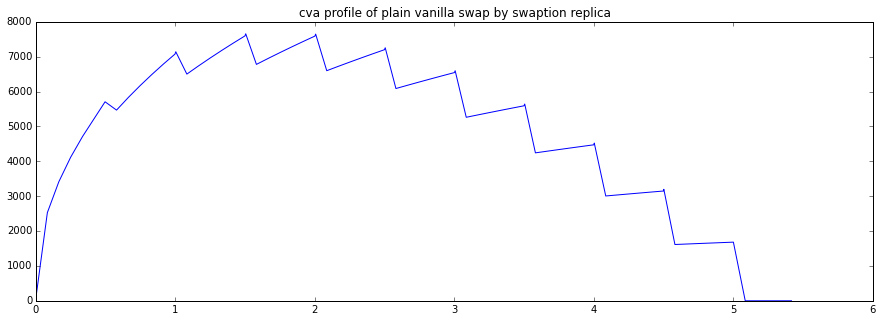
\includegraphics[scale=.4]{img/profile_1.png} 
\end{center}
\end{frame}
%...................................................................................................
\begin{frame}{Exposure Profile: Value Density}
\begin{center}
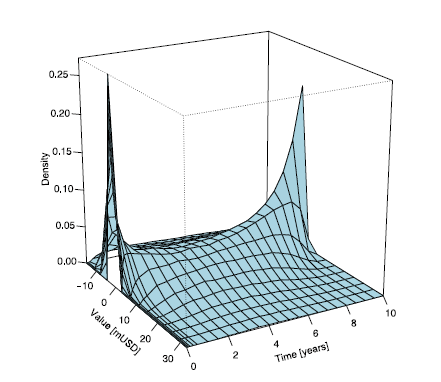
\includegraphics[scale=.8]{img/profilo_3.png} 
\end{center}
\end{frame}
%...................................................................................................
\begin{frame}{Exposure Profile}
\noindent\begin{minipage}{0.5\textwidth}% adapt widths of minipages to your needs
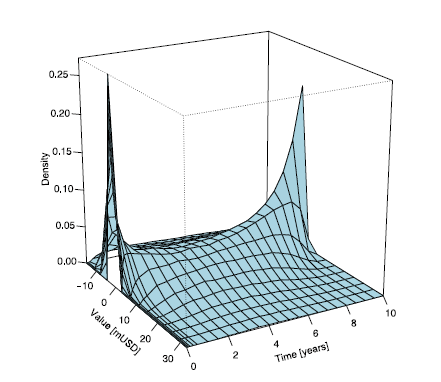
\includegraphics[width=\linewidth]{img/profilo_3.png}
\end{minipage}%
\hfill%
\begin{minipage}{0.5\textwidth}
\begin{itemize}
\item Figure  shows  the full price distribution over time.
\item The fair value for the swap, and this must therefore have
value (and hence exposure level) identically equal to zero at inception. 
\item Similarly,
towards the end of the transaction, when all payments but one due under the swap
have been paid, the exposure remaining is that from only a single coupon exchange.
\end{itemize}
\end{minipage}
\end{frame}
%...................................................................................................
\begin{frame}{Exposure Profile}
\noindent\begin{minipage}{0.5\textwidth}% adapt widths of minipages to your needs
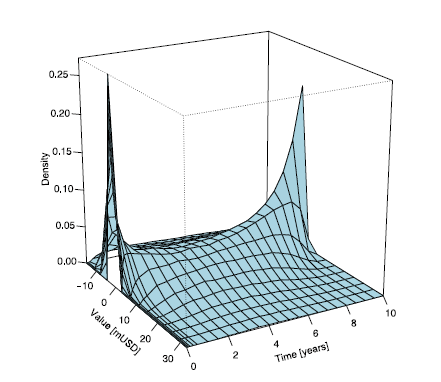
\includegraphics[width=\linewidth]{img/profilo_3.png}
\end{minipage}%
\hfill%
\begin{minipage}{0.5\textwidth}
\begin{itemize}
\footnotesize
\item This explains what happens at the right end of the profile. 
\item At intermediate times, the
shape of the profile is the result of opposing effects. 
\item On the one hand, as the interest
rates underlying the swap diffuse, there is more variability in the realised Libor rates,
potentially leading to higher exposure. 
\item On the other hand, as time evolves there are
fewer payments remaining under the swap, and this mitigates the effect of diffusing
rates.
\normalsize
\end{itemize}
\end{minipage}
\end{frame}
%...................................................................................................
\begin{frame}{Exposure Profiles}
\begin{itemize}
\item So there are two main effects that determine the credit exposure over time for a single transaction or for a portfolio of transactions with the same counterparty: diffusion and amortization;
\item as time passes, the "diffusion effect" tends to increase the exposure, since there is greater variability and, hence, greater potential for market price factors to move significantly away fro current levels;
\item the "amortization effect", in contrast, tends to decrease the exposure over time, because it reduces the remaining cash flows that are exposed to default;
\end{itemize}
\end{frame}
%...................................................................................................
\begin{frame}{Exposure Profiles}
\begin{itemize}
\item For single cash flow products, such as FX Forwards, the potential exposure peaks at the maturity of the transaction, because it is driven purely by "diffusion effect";
\item on the other hand, for products with multiple cash flows, such as interest-rate swaps, the potential exposure usually peaks at one-third to one-half of the way into the life of the transaction;
\end{itemize}
\end{frame}
%...................................................................................................
\begin{frame}{Credit Value Adjustment}
\begin{itemize}
\item \textbf{Credit Value Adjustment (CVA)} is by definition the difference between the risk-free portfolio value and the true portfolio value that takes into account the possibility of a counterparty's default;
\item in other words CVA is the market value of counterparty credit risk; 
\end{itemize}
\end{frame}
%...................................................................................................
\begin{frame}{Credit Value Adjustment}
\begin{itemize}
\item Assuming independence between exposure and counterparty's credit quality greatly simplifies the analysis. 
\item under this assumption we can write
\begin{equation}\label{definizione CVA}
CVA= (1-R) \int\limits_0^T EE^\star (t) dPD(0,t)
\end{equation}
where $EE^\star (t)$ is the risk-neutral discounted expected exposure (EE) given by
\begin{equation}\label{definizione EE}
EE^\star (t) = E^Q \left[ \frac{B_0}{B_t} E(t) \right]
\end{equation}
\end{itemize}
\end{frame}
%...................................................................................................
\begin{frame}{Credit Value Adjustment}
\begin{itemize}
\item In general calculating discounted EE requires simulations;
\item Exposure is simulated at a fixed set of simulation dates, therefore the integral in \eqref{definizione CVA} has to be approximated by the sum:
\begin{equation}\label{definizione CVA discreta}
CVA = (1-R) \sum\limits_{i=1}^N EE^\star (t_k) PD(t_{k-1},t_k)
\end{equation} 
\item Since expectation in \eqref{definizione EE} is risk-neutral, scenario models for all price factors should be arbitrage free;
\item This is achieved by appropriate calibration of drifts and volatilities specified in the price-factor evolution model;
\end{itemize}
\end{frame}
%...................................................................................................
%...................................................................................................
\subsection{CVA of a Plain Vanilla Swap: the Analytical Model}
%...................................................................................................
%...................................................................................................
%...................................................................................................
\begin{frame}{The General Unilateral Counterparty Risk Pricing Formula}
\begin{itemize}
\item At valuation time $t$, and provided the counterparty has not defaulted before $t$, i.e. on $\{ \tau > t \}$, the price of our payoff with maturity $T$ under counterparty risk is

\begin{equation}
\begin{split}
\mathbb{E}_t [\bar \Pi (t, T) ] &=  \mathbb{E}_t [\Pi (t, T) ]  - 
\underbrace{
\mathbb{E}_t [ LGD \, \mathbb{I}_{t \le \tau \le T} D(t, \tau) (NPV(\tau))^+ ]  
}_\text{positive counterparty-risk adjustment} \\
&= \mathbb{E}_t [\Pi (t, T) ]  - U_{CVA}(t,T)
\end{split}
\end{equation}
with
\begin{equation}
\begin{split}
U_{CVA}(t,T) &= \mathbb{E}_t [ LGD \, \mathbb{I}_{t \le \tau \le T} D(t, \tau) (NPV(\tau))^+ ] \\
&= \mathbb{E}_t [ LGD \, \mathbb{I}_{t \le \tau \le T} D(t, \tau) EAD ]
\end{split}
\end{equation}
Where $LGD = 1 - REC$ is the loss given default, and the recovery fraction $REC$ is assumed to be deterministic. 
\end{itemize}
\end{frame}
%...................................................................................................
\begin{frame}{The General Unilateral Counterparty Risk Pricing Formula}
\begin{itemize}
\item It is clear that the value of a defaultable claim is the sum of the value of the corresponding default-free claim minus a positive adjustment. 
\item The positive adjustment to be subtracted is called (Unilateral) Credit Valuation Adjustment (CVA), and it is given by a call option (with zero strike) on the residual NPV at default, giving nonzero contribution only in scenario where $\tau \le T$.
\end{itemize}
\end{frame}
%...................................................................................................
\begin{frame}{The General Unilateral Counterparty Risk Pricing Formula}
\begin{itemize}
\item Counterparty risk thus adds and optionality level to the original payoff. 
\item This renders the counterparty risk payoff model dependent even when the original payoff is model independent. \item This implies, for example, that while the valuation of swaps without counterparty risk is model independent, requiring no dynamical model for the term structure (no volatility and correlations in particular), the valuation of swaps under counterpaty risk will require and interest rate model. 
\end{itemize}
\end{frame}
%...................................................................................................
\begin{frame}{The General Unilateral Counterparty Risk Pricing Formula}
\begin{itemize}
\item Now we explore the well known result that the component of the IRS price due to counterparty risk is the sum of swaption prices with different maturities, each weighted with the probability of defaulting around that maturity. 
\item Let us suppose that we are a default free counterparty "B" entering a payer swap with a defaultable counterparty "C", exchanging fixed for floating payments at times $T_{a+1},\dots,T_b$. 
\item Denote by $\beta_i$ the year fraction between $T_{i-1}$ and $T_i$, and by $P(t, T_i)$ the default-free zero coupon bond price at time $t$ for maturity $T_i$. We take a unit notional on the swap. 
\item The contract requires us to pay a fixed rate $K$ and to receive the floating rate $L$ resetting one period earlier until the default time $\tau$ of "B" or until final maturity $T$ if $\tau > T$. 
\item The fair forward-swap rate $K$ at a given time $t$ in a default-free market is the one which renders the swap zero-valued in $t$. 
\end{itemize}
\end{frame}
%...................................................................................................
\begin{frame}{The General Unilateral Counterparty Risk Pricing Formula}
\begin{itemize}
\item In the risk-free case the discounted payoff for a payer IRS is

\begin{equation}
\sum\limits_{i=a+1}^b  D(t,T_i) \beta_i (L(T_{i-1},T_i) -K)
\end{equation}

\item and the forward swap rate rendering the contract fair is

$$
K=S(t; T_a,T_b) = S_{a,b} (t) = \frac{P(t,T_a) - P(t,T_b)}{\sum\limits_{i=a+1}^b  P(t,T_i) \beta_i}
$$
\end{itemize}
\end{frame}
%...................................................................................................
\begin{frame}{The General Unilateral Counterparty Risk Pricing Formula}
\begin{itemize}
\item Of course if we consider the possibility that "C" may default, the correct spread to be paid in the fixed leg is lower as we are willing to be rewarded for bearing this default risk. 
\item In particular we have
\begin{equation}
\begin{split}
U_{CVA}(t,T_b) &= LGD \> \mathbb{E}_t [ \mathbb{I}_{\tau \le T_b} D(t,\tau) (NPV(\tau))^+ ] \\
&= LGD \> \int\limits_{T_a}^{T_b} PS \left( t;s,T_b,K,S(t;s,T_b), \sigma_{s,T_b} \right) \> d_s \mathbb{Q} \{\tau \le s \}
\end{split}
\end{equation}
being $PS \left( t;s,T_b,K,S(t;s,T_b), \sigma_{s,T_b} \right) $ the price in $t$ of a swaption with maturity $s$, strike $K$ underlying forward swap rate $S(t;s,T_b)$, volatility $\sigma_{s,T_b}$ and underlying swap with final maturity $T_b$.
\end{itemize}
\end{frame}
%...................................................................................................
\begin{frame}{The General Unilateral Counterparty Risk Pricing Formula}
\begin{itemize}
\item The proof is the following: given independence between $\tau$ and the interest rates, and given that the residual NPV is a forward start IRS starting at the default time, the option on the residual NPV is a sum of swaptions with maturities ranging the possible values of the default time, each weighted (thanks to the independence assumption) by the probabilities of defaulting around each time value. 
\item We can simplify formulas allow the default to happen only at points $T_i$ of the fixed leg payment grid. 
\item In this way the expected loss part is simplified. 
\end{itemize}
\end{frame}
%...................................................................................................
\begin{frame}{The General Unilateral Counterparty Risk Pricing Formula}
\begin{itemize}
\item Indeed in the case of postponed (default occour to the first $T_i$ following $\tau$) payoff we obtain:
\footnotesize
\begin{equation}
\begin{split}
U_{CVA}(t,T_b) &= LGD \> \mathbb{E}_t [ \mathbb{I}_{\tau \le T_b} D(t,\tau) (NPV(\tau))^+ ] \\
&= LGD \> \sum\limits_{i=a+1}^{b-1} PS \left( t;s,T_b,K,S(t;s,T_b), \sigma_{s,T_b} \right) 
\> \left( \mathbb{Q} \{\tau \ge T_i \} - \mathbb{Q} \{\tau > T_i \} \right)
\end{split}
\end{equation}
\normalsize
\end{itemize}
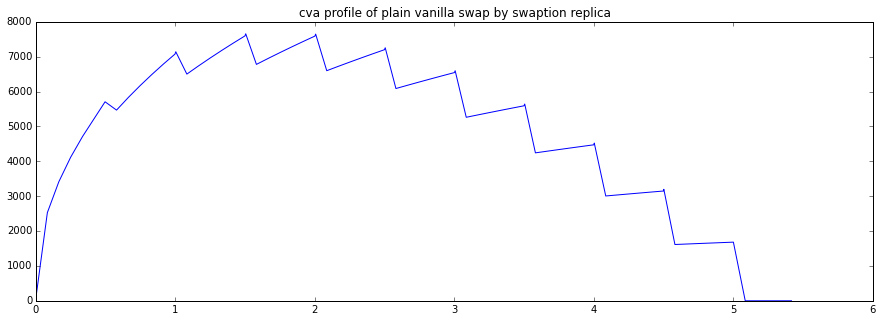
\includegraphics[scale=.4]{img/profile_1.png} 
\end{frame}
%...................................................................................................
\begin{frame}{Notebook}
\noindent\begin{minipage}{0.5\textwidth}% adapt widths of minipages to your needs

\includegraphics[width=\linewidth]{img/exercise.jpg}
\end{minipage}%
\hfill%
\begin{minipage}{0.5\textwidth}
\begin{itemize}
\item {\bf GitHub        : }    polyhedron-gdl;
\item {\bf Notebook   : }    n09\_cva\_swap;
\end{itemize}
\end{minipage}
\end{frame}
%...................................................................................................
%...................................................................................................
\subsection{CVA of a Plain Vanilla Swap: the Simulation Approach}
%...................................................................................................
%...................................................................................................
%...................................................................................................
\begin{frame}{Monte Carlo Framework for CVA}
The industry practice to compute exposure is to use a simple Monte Carlo framework
implemented in three steps: 
\begin{enumerate}
\item scenario generation, 
\item pricing
\item  aggregation.
\end{enumerate} 
\end{frame}
%...................................................................................................
\begin{frame}{Monte Carlo Framework for CVA}
\begin{itemize}
\item The first step involves generating scenarios of the underlying risk factors at future
points in time. 
\item Simple products can then be priced on each scenario and each time
step, therefore generating empirical price distributions. 
\item From the price distribution
at each time it is then possible to extract convenient statistical quantities. 
\item Exposure
of portfolios can be computed by consistently pricing different products on the same
underlying scenarios and aggregating the results taking into account possible netting
and collateral agreement with the counterparty.
\end{itemize}
\end{frame}
%...................................................................................................
\begin{frame}{Monte Carlo Framework for CVA}
\begin{itemize}
\item If taken literally, this approach works only for relatively simple products which
can be priced analytically, or which can be approximated in analytical form, and
which do not need complex calibrations depending on market scenarios. 
\item More exotic
products requiring relatively complex pricing, cannot be treated in this way. 
\end{itemize}
\end{frame}

%...................................................................................................
\begin{frame}{CVA of a Plain Vanilla Swap: the Simulation Approach}
\begin{enumerate}
\item Simulate yield curve at future dates
\item Calculate your derivatives portfolio NPV (net present value) at each time point for each scenario
\item Calculate CVA as sum of Expected Exposure multiplied by probability of default at this interval

$$ CVA=(1-R) \int DF(t)EE(t)dQ_t $$

where $R$ is the Recovery Rate (normally set to 40\%) $EE(t)$ is the expected exposure at time $t$ and $dQ_t$ the survival probability density, $DF(t)$ is the discount factor at time $t$.

\end{enumerate}
\end{frame}
%...................................................................................................
\begin{frame}{CVA of a Plain Vanilla Swap: the Simulation Approach}
\begin{itemize}
\item In this simple example we will use a modified version of Hull White model to generate future yield curves. In practice many banks use some yield curve evolution models based on this model. 
\item For each point of time we will generate whole yield curve based on short rate. Then we will price our interest rate swap on each of these curves;
\item To approximate CVA we will use BASEL III formula for regulatory capital charge approximating default probability [or survival probability ] as $exp(-S_T/(1-R))$ so we get
\footnotesize
$$
CVA=(1-R) \sum\limits_i \frac{EE(T_i)^\star + EE(T_{i-1}^\star}{2}
\left( e^{-S(T_{i-1})/(1-R)}-e^{-S(T_i)/(1-R)} \right)
$$
\normalsize
where $EE^\star$ is the discounted Expected Exposure of portfolio.
\end{itemize}
\end{frame}
%...................................................................................................
\begin{frame}{CVA of a Plain Vanilla Swap: the Simulation Approach}
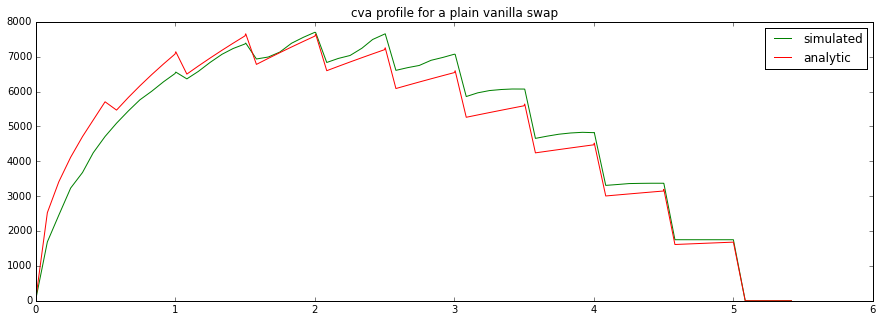
\includegraphics[scale=.4]{img/profilo_2.png} 
\end{frame}
%...................................................................................................
\begin{frame}{Notebook}
\noindent\begin{minipage}{0.5\textwidth}% adapt widths of minipages to your needs

\includegraphics[width=\linewidth]{img/exercise.jpg}
\end{minipage}%
\hfill%
\begin{minipage}{0.5\textwidth}
\begin{itemize}
\item {\bf GitHub        : }    polyhedron-gdl;
\item {\bf Notebook   : }    n10\_mcs\_cva\_swap;
\end{itemize}
\end{minipage}
\end{frame}
%...................................................................................................
\begin{frame}{Implementation Challenges}
\begin{itemize}
\item The Monte Carlo framework we have shown in the previous section, seems to give
a good implementation recipe. 
\item For a given portfolio of transactions we could 
identify the underlying risk factors and simulate forward (or spot) prices, taking
into account correlations if required, use functions already implemented to price
each product, and then  derive statistical quantities. 
\item As we have mentioned already,
this could be the approach followed by a financial institution to assess the
counterparty credit risk of its OTC derivatives portfolios.
\end{itemize}
\end{frame}
%...................................................................................................
\begin{frame}{Implementation Challenges}
\begin{itemize}
\item In the implementation phase, however, there can be issues which need to be addressed.
\item The generation of correlated scenarios is not trivial, as there can be thousands
of different risk factors driving the dynamics of products in the portfolio. 
\item Consider
for example an equity portfolio, where each underlying stock needs, at
least in principle, a specific simulation.
\end{itemize}
\end{frame}
%...................................................................................................
\begin{frame}{Implementation Challenges}
\begin{itemize}
\item Not all products can be computed in analytical form. 
\item Most exotics are priced
on grids using PDEs or using Monte Carlo approaches.
\item In these cases the exposure
computation would require a Monte Carlo simulation for scenarios and
a Monte Carlo simulation, or a PDE computation, for each scenario and time
step to price the instrument. 
\item This becomes quickly unfeasible from a computational
point of view. 
\item In addition, depending on the model used for pricing,
calibration could also become problematic, as it has to be performed at each
scenario.
\end{itemize}
\end{frame}
%...................................................................................................
\begin{frame}{American Monte Carlo}
\begin{itemize}
\item The points highlighted in the previous section clearly show that the classical Monte
Carlo scheme has intrinsic limitations and that we need an alternative approach. 
\item There are possibilities to circumvent in
a systematic way some of the problems related to valuation and architecture.
\item The basic idea is to approach the counterparty exposure problem as a pricing
problem, and thus to use pricing algorithms, which generate not just the value of a
trade at inception, but rather a price distribution at predetermined time steps. 
\item One
possibility is to use the so called American Monte Carlo algorithm, which we will
refer to as, simply, the AMC algorithm.
\item  The main feature of this algorithm is that,
instead of building a price moving forward in time, it starts from maturity, where
the value of the transaction is known, and goes backwards, till the inception.
\end{itemize}
\end{frame}
%...................................................................................................
\begin{frame}{AMC CVA Simulation}
\begin{center}
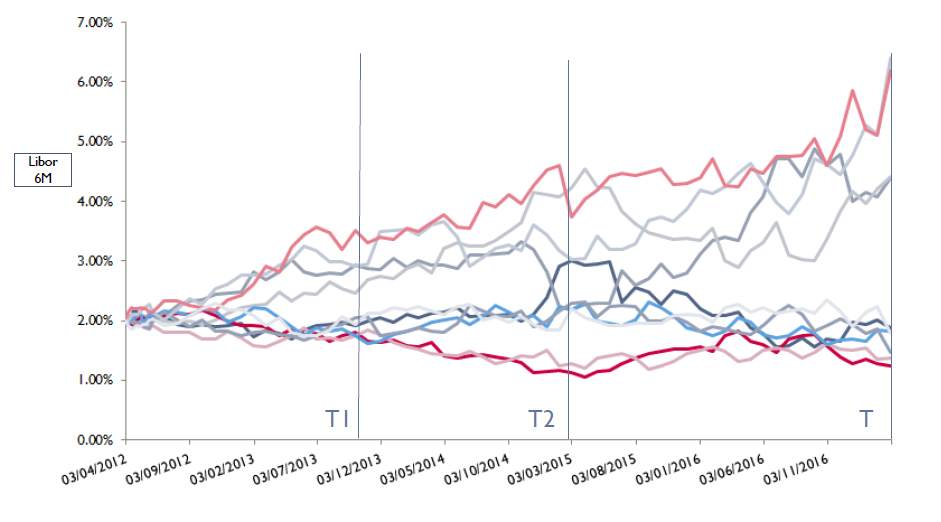
\includegraphics[scale=.4]{img/AMC1.PNG} 
\end{center}
\begin{itemize}
\scriptsize
\item Let's illustrate with a Bermuda Swaption which can be exercised at 2 dates, T1 and T2. 
\normalsize
\end{itemize}
\end{frame}
%...................................................................................................
\begin{frame}{AMC CVA Simulation}
\begin{center}
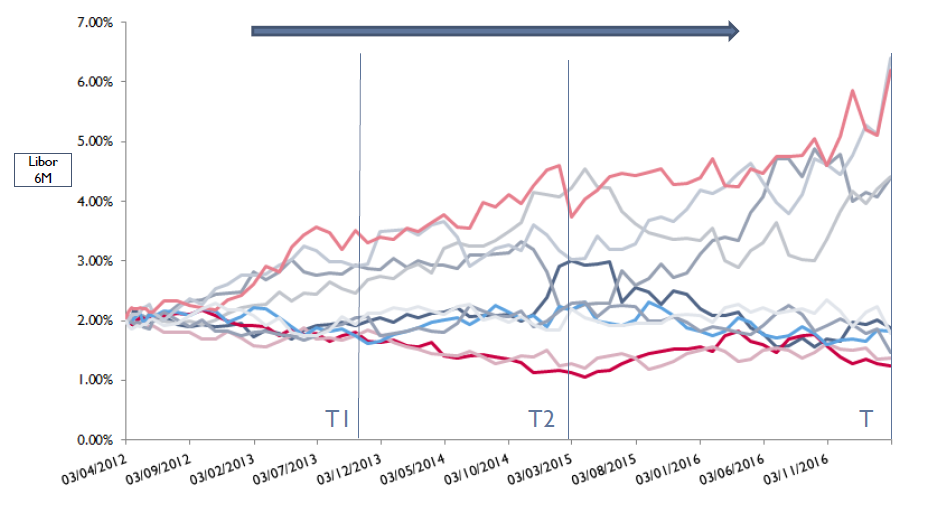
\includegraphics[scale=.4]{img/AMC2.PNG} 
\end{center}
\begin{itemize}
\scriptsize
\item Forward Phase: we diffuse risk factors and store in memory contract cash flows and payoff variables as the will be used in the Backward Phase.
\normalsize
\end{itemize}
\end{frame}
%...................................................................................................
\begin{frame}{AMC CVA Simulation}
\begin{center}
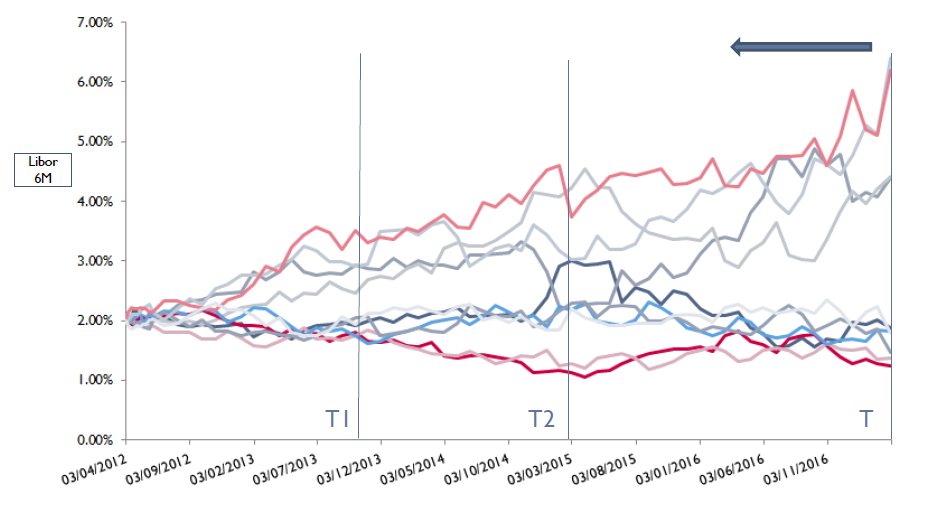
\includegraphics[scale=.4]{img/AMC3.PNG} 
\end{center}
\begin{itemize}
\scriptsize
\item Backward Phase: we discount payoff contract and add cash flows up to T2. 
\normalsize
\end{itemize}
\end{frame}
%...................................................................................................
\begin{frame}{AMC CVA Simulation}
\begin{center}
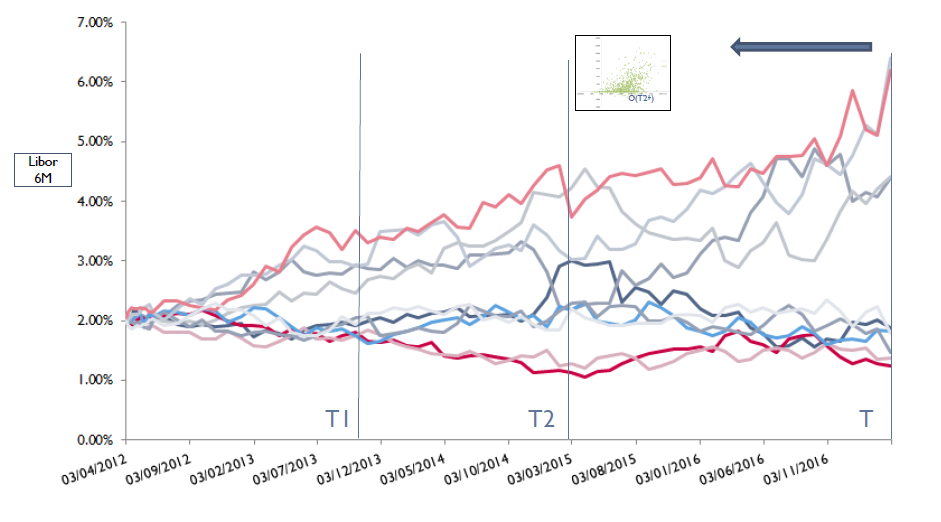
\includegraphics[scale=.4]{img/AMC4.PNG} 
\end{center}
\begin{itemize}
\scriptsize
\item Backward Phase: At T2 we obtain a cloud of points... 
\normalsize
\end{itemize}
\end{frame}
%...................................................................................................
\begin{frame}{AMC CVA Simulation}
\begin{center}
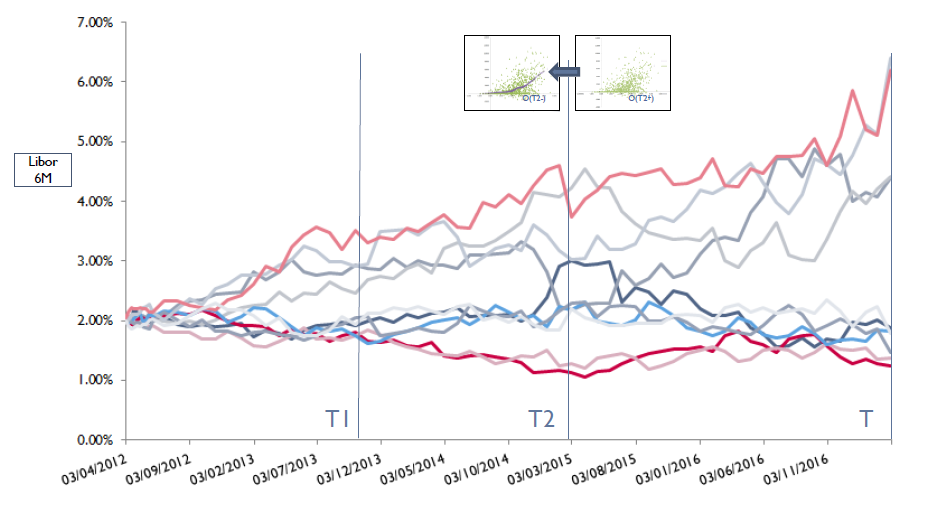
\includegraphics[scale=.4]{img/AMC5.PNG} 
\end{center}
\begin{itemize}
\scriptsize
\item ... regression is performed to obtain product fair value at T2 as a function of regression basis. 
\normalsize
\end{itemize}
\end{frame}
%...................................................................................................
\begin{frame}{AMC CVA Simulation}
\begin{center}
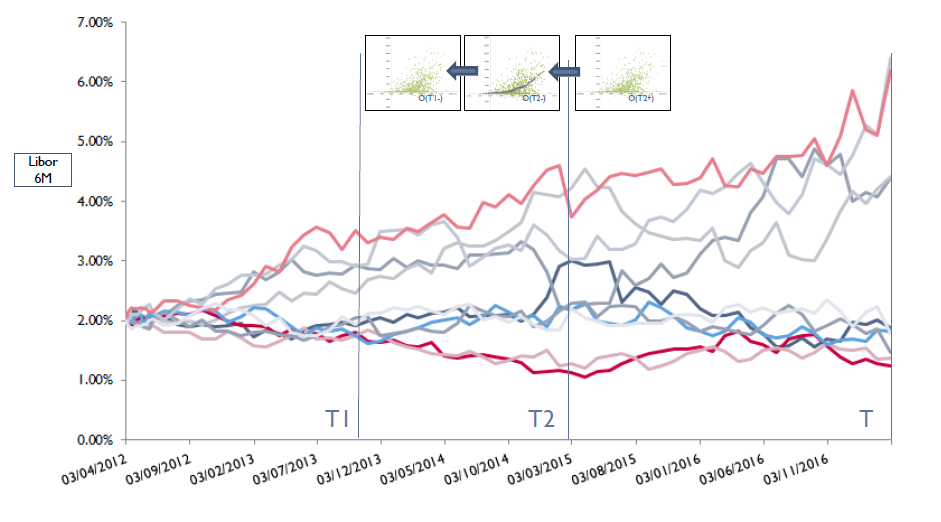
\includegraphics[scale=.4]{img/AMC6.PNG} 
\end{center}
\begin{itemize}
\scriptsize
\item We discount to T1 obtaining a cloud of points (adding present cash flow from forward phase). 
\normalsize
\end{itemize}
\end{frame}
%...................................................................................................
\begin{frame}{AMC CVA Simulation}
\begin{center}
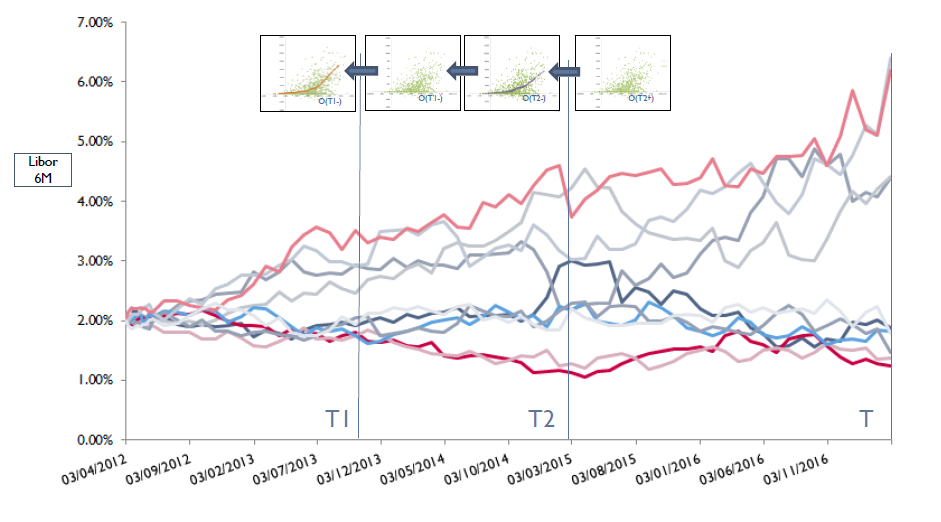
\includegraphics[scale=.4]{img/AMC7.PNG} 
\end{center}
\begin{itemize}
\scriptsize
\item  Regression is performed at T1 as a function of regression basis. 
\normalsize
\end{itemize}
\end{frame}
%...................................................................................................
\begin{frame}{AMC CVA Simulation}
\begin{center}
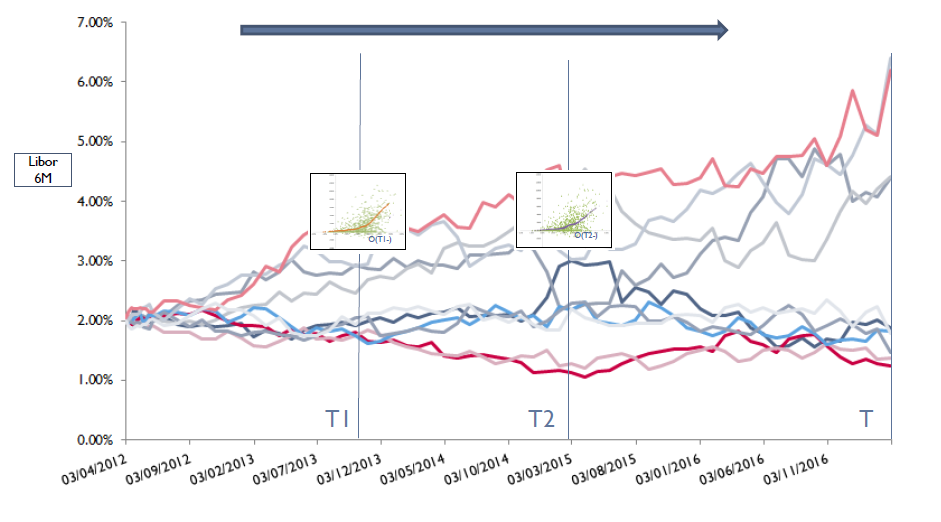
\includegraphics[scale=.4]{img/AMC8.PNG} 
\end{center}
\begin{itemize}
\scriptsize
\item Forward Phase: we then move forward again and invoke regression functions with the new set of MC paths ... 
\normalsize
\end{itemize}
\end{frame}
%...................................................................................................
\begin{frame}{AMC CVA Simulation}
\begin{center}
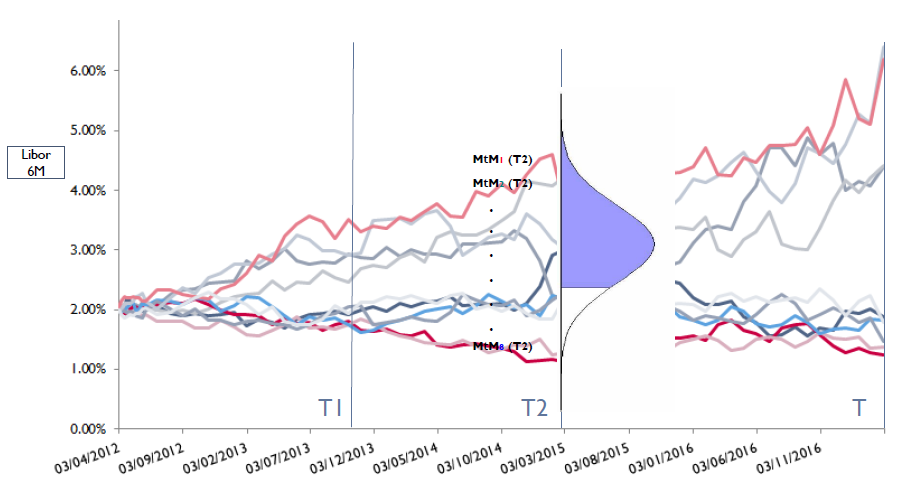
\includegraphics[scale=.4]{img/AMC9.PNG} 
\end{center}
\begin{itemize}
\scriptsize
\item We can compute distribution of MTMs, exposure, EPE, PFE, etc... 
\normalsize
\end{itemize}
\end{frame}
%...................................................................................................
\begin{frame}{AMC CVA Simulation}
Recap
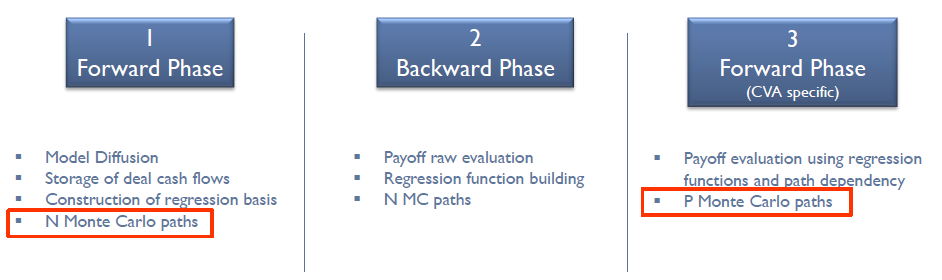
\includegraphics[scale=.5]{img/AMC10.PNG} 
\begin{itemize}
\item \textbf{Important Remark}: In Phase 3, MC diffusion can be different from Phase 1.
\end{itemize}
\end{frame}
%===================================================================================================
%...................................................................................................
\begin{frame}{Credits}
\begin{itemize}
\item Damiano Brigo, Fabio Mercurio "Interest Rate Models — Theory and Practice" Springer Finance (2006)
\item Damiano Brigo, Massimo Morini, Andrea Pallavicini "Counterparty Credit Risk, Collateral and Funding" Wiley Finance (2013)
\item Umberto Cherubini, Elisa Luciano, Walter Vecchiato "Copula Methods in Finance" Wiley Finance (2004)
\item Tommaso Gabbriellini "American Options with Monte Carlo" Presentation on Slideshare
\item Yves Hilpisch "Derivatives Analytics with Python" Wiley Finance (2015) 
\item Don L. McLeish "Monte Carlo Simulation and Finance" Wiley Finance (2005)
\end{itemize}
\end{frame}

\end{document}




